\chapter{Les galaxies}
\label{sec:galaxies}

Les étoiles se forment rarement de manière isolée mais généralement par paquet que l'on nomme galaxies.
Ces zones ont une densité de gaz particulièrement élevée, et disposent donc de suffisamment de matériaux pour amorcer la formation stellaire.
Comme la densité de gaz suit la distribution de matière noire, c'est grâce a cette dernière que l'on détecte les galaxies.
L'idée est d'utiliser un halo finder pour détecter les surdensités de matière noire.
On cherchera ensuite a associer les baryons aux halos.

Nous verrons dans cette partie différentes propriétés des baryons en fonction de la masse de leur halo hôte.
Nous regarderons des propriétés telle la fraction de masse baryonique ou le taux de formation stellaire.

%L'étude des simulation se fait souvent halos par halos.
%Quand on cherche a déterminer es propriétés des galaxies, un paramètre important est leur masse.
%Comme le gaz suit la dynamique des baryons, les galaxies sont situées dans les surdensités de matière noire.

\section{La détection des halos}
La première étape est de détecter les halos.
L'objectif d'un halo finder est de détecter les surdensités dans le champs de matière noire.
Comme nous l'avons vu plus tôt (voir sec \ref{sec:solverDM}), le champ de matière noire utilise une représentation sous forme de particules.

J'ai principalement utilisé l’algorithme Friend Of Friend (FOF) pour détecter les sur-densités et plus particulièrement pFOF l'implémentation parallèle de \cite{2014A&A...564A..13R}.
pFOF lie les particules regroupées en surdensité, en utilisant une taille de lien caractéristique.
Il retourne ensuite une liste de groupes de particules et une liste de positions déterminées par le centre de masse des particules de chaque halos.

%FOF retourne une liste de position de halo, une liste permettant de lier les particules détecté aux halos.
Il existe plusieurs possibilités pour ensuite déterminer l'étendue spatiale des halos.

\subsection{Le rayon de Viriel}
La première possibilité pour déterminer l'étendue spatiale du halo consiste a utiliser l'approximation du $R_{200}$ \citep{1997ApJ...490..493N}.
Elle consiste à considérer une sphère aillant une densité moyenne de $200$ fois la densité moyenne de l'univers $\bar{\rho}$.

\begin{equation}
R_{200}= \left( \frac{3\cdot M_{FoF} }{4\pi\cdot 200 \bar{\rho}} \right)^{1/3}
\end{equation}


\subsection{Association dans le R$_{200}$}

%Il faut ensuite y associer les autres champs physique contenus par la grille 
%La première méthode consiste a utiliser l'approximation du R200.
%Il faudra associer, la matière noire, le gaz et les étoiles compris a l'intérieur d'une sphere de rayon R200.

%Il faut ensuite y associer les autres champs physique contenus par la grille 

%Le méthode est la suivante:
%
%\begin{itemize}
%\item générer un KDtree sur les particule de matière noire / les étoiles / la grille AMR
%\item Faire une recherche sphérique autour de la positions des halo, sur un rayon de R200
%\item stocker les indices dans une structure
%\end{itemize}

Nous avons donc a ce stade une position et une étendue pour chaque halo.
On cherchera ensuite a y associer les galaxies (surdensité d'étoiles).
J'ai utilisé un KD-tree, généré sur les étoiles, pour faire des recherches sphérique de manière efficace.

Nous chercherons également a obtenir des informations sur les champs physique contenus pas la grille AMR.
Il sera possible d'utiliser un KDtree pour déterminer quelles sont les cellules qui se trouvent dans le $R_{200}$ du halo.
IL suffi pour cela d'utiliser les centres de cellule a la place de la position des étoiles.
%Comme les particules de matière noire  données par FoF ne represente pas le meme volume, dans un soucis de cohérence, on appliquera cette méthodes a la matière noire également.
A ce stade nous avons donc la possibilité, pour chaque halo, de connaître n'importe qu'elle grandeurs comprissent dans son $R_{200}$.

Pour les petits halos, peu résolus, la taille des cellules peu être grandes par rapport au $R_{200}$.
Pour minimiser l'erreur commise, la grille AMR pourra être projeter sur une grille régulière de résolution arbitraire.
Cette méthode permettra d'associer des sous parties de cellules aux halo et améliorera la precision global de l'association.

\subsection{Le problème de la forme des halos}

%Fortement non viriallisé a z=6\\
%beaucoup de dynamique et merger dans les filemments

L'approximation du $R_{200}$ est valide et a fait ses preuves dans le cas de halos virialisés.  %TODO ref
Cependant, a haut redshift (z>5) les halos sont encore en formation et peuvent être fortement non virialisé.
Il devient alors difficile pour FOF de séparer les différentes sous parties d'une même sur-densité.
La figure \ref{fig:part_halo} illustre particulièrement bien ce problème de détection.

La sur-densité détectée par \ac{FOF} est loin d'être sphérique, et l'approximation du $R_{200}$ n'est pas valide dans ce cas.
Du fait de l'effondrement hiérarchique de la matière noire, changer la longueur de lissage ne changera pas le problème et ne ferait que le reporter a d'autres échelles.


\begin{figure}[bth]
        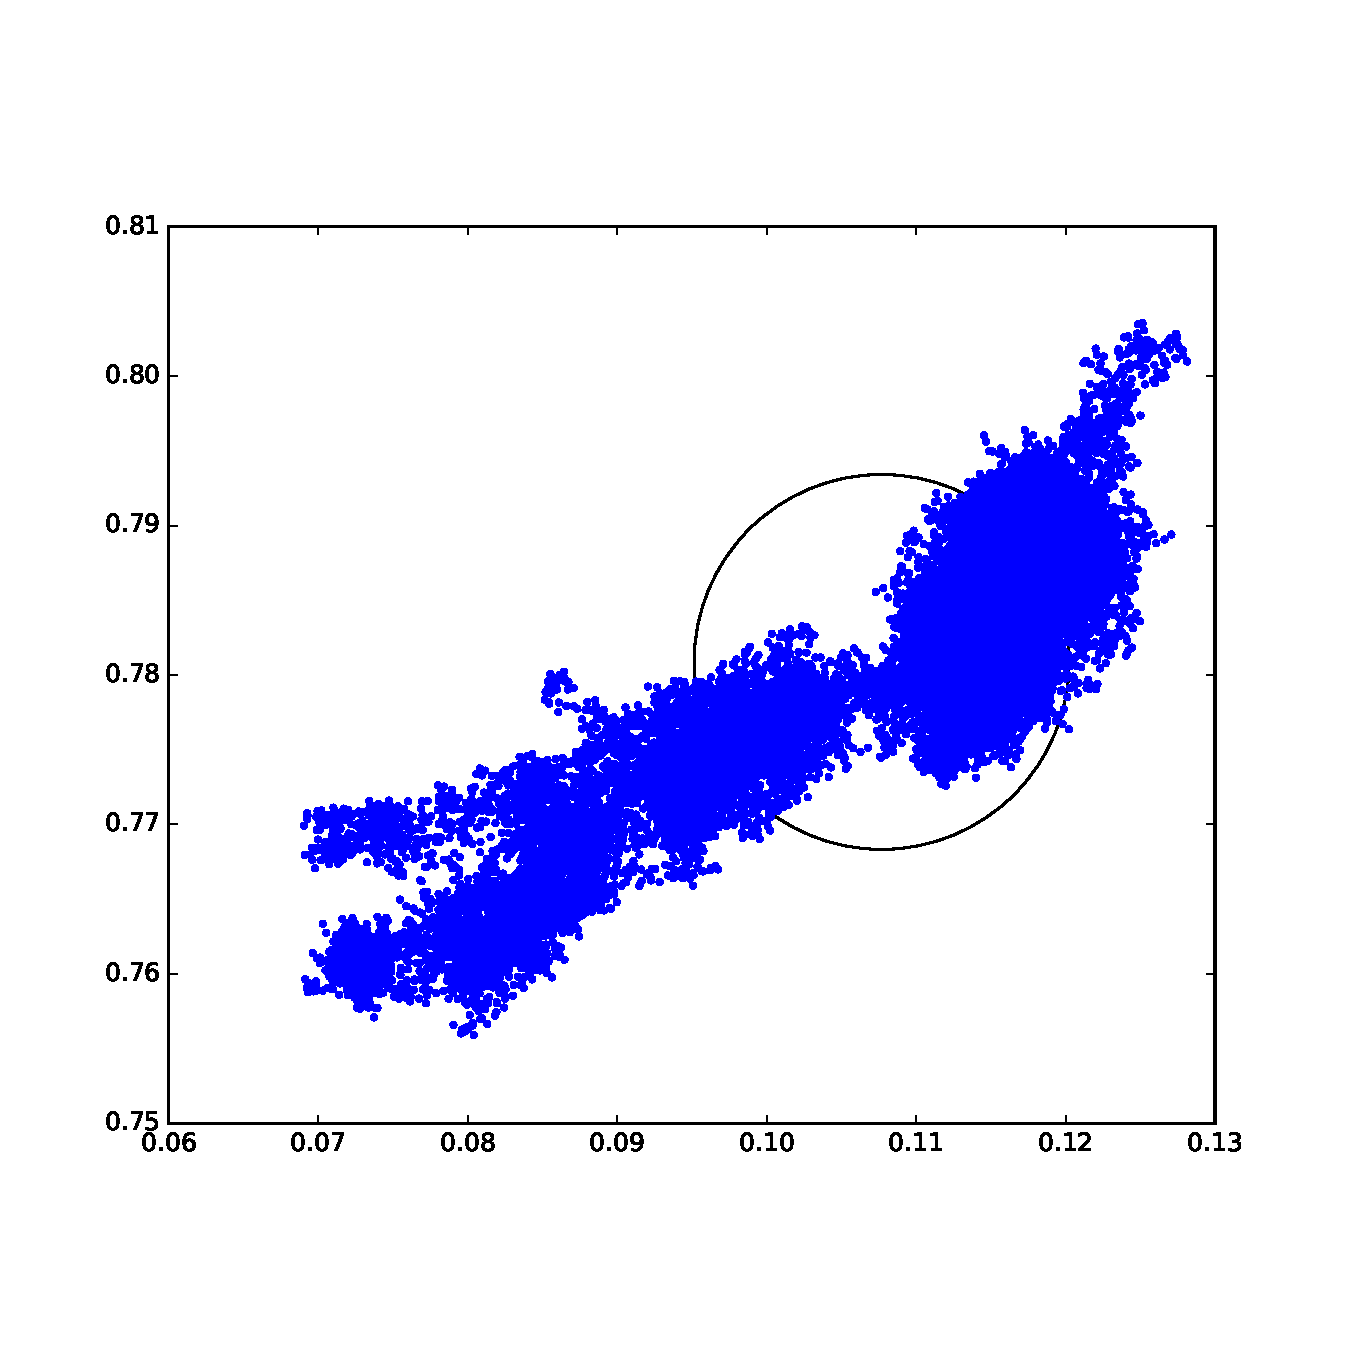
\includegraphics[width=.95\textwidth]{img/03/part_halo_R200.pdf} 
        \caption{La détection des halos par FOF peux être difficile au moment de la réionisation car les structure peuvent ne pas être virialisée.
        }
 		\label{fig:part_halo}
\end{figure}


\subsection{Association "fine"}

Dans le but d'améliorer ces problèmes d'identification dans les halos fortement non virialisé, j'ai développé une méthode pour associer plus précisément les halos et la grille.
Cette méthode consiste a rechercher, pour chaque particule de matière noire, sa plus proche cellule.
Malgré que cette recherche soit effectué de manière efficace a l'aide d'un KD tree, cette méthode est évidemment bien plus longue qu'une simple recherche dans la sphere.

%\begin{itemize}
%\item générer un KDtree sur la grille
%\item pour chaque particule d'une halo, trouver la plus proche cellule
%\item filtrer les cellules doublons
%\end{itemize}

La figure \ref{fig:R200_fine} présente la détection des cellule entre les deux méthodes pour le halo de la figure \ref{fig:part_halo}.


\begin{figure}[bth]
	\subfloat[]{		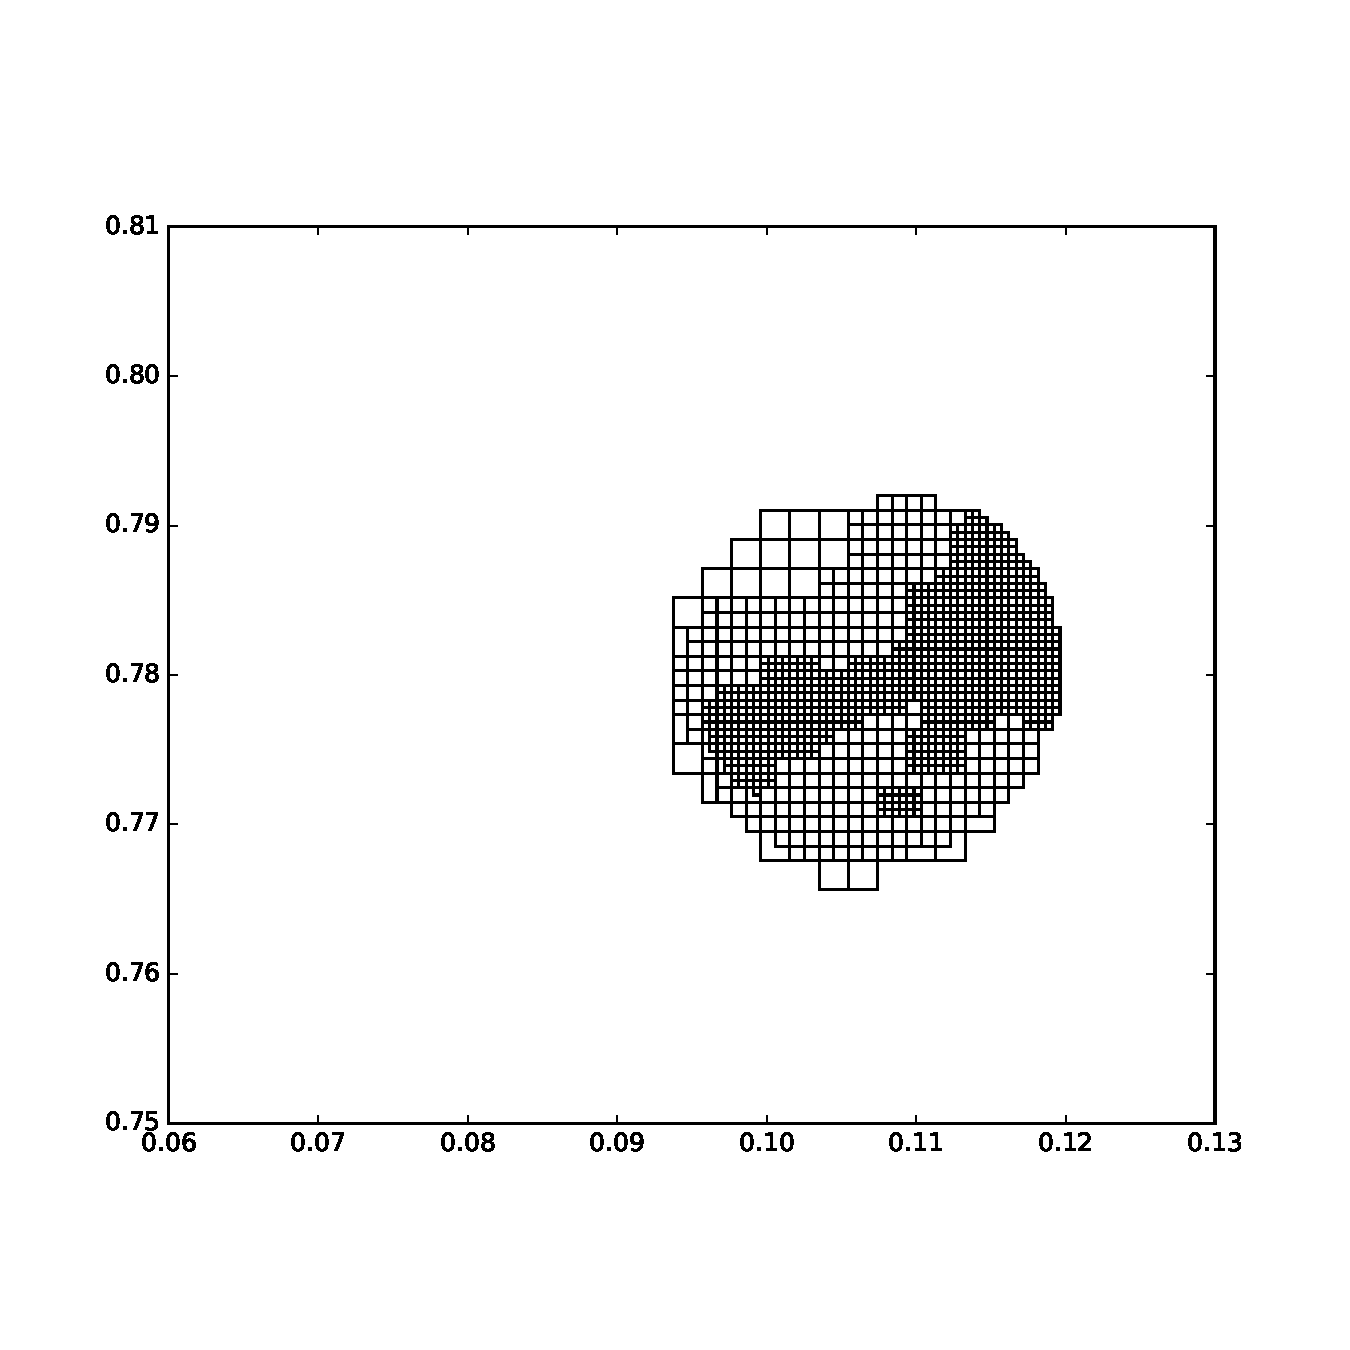
\includegraphics[width=.45\linewidth]{img/03/part_cells.pdf} }
	\subfloat[]{		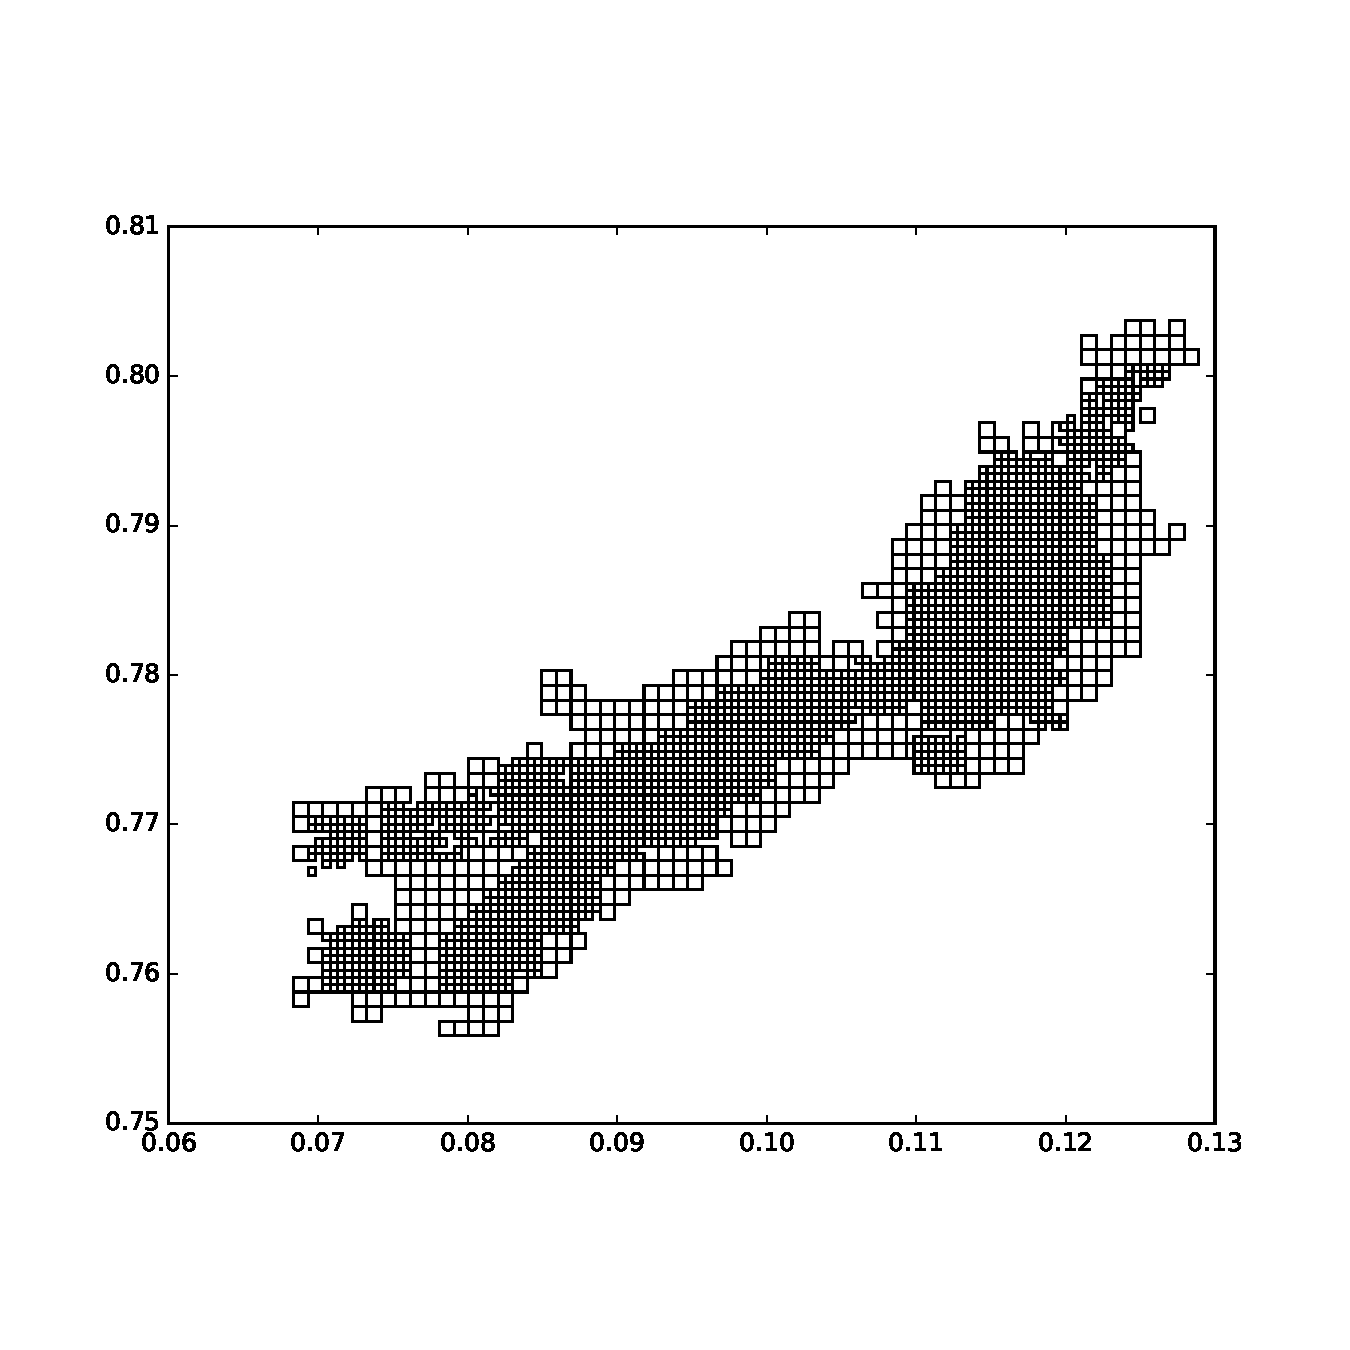
\includegraphics[width=.45\linewidth]{img/03/part_cells_fine.pdf} }
        \caption{Cellule associées au halo dans le cas de l'estimation R200 vs dans le cas de la méthode fine.
        }
 		\label{fig:R200_fine}
\end{figure}




\section{Étude de la composition des halos}

Maintenant que nous pouvons associer toutes la physique au sein de chaque halo, nous pouvons regarder  différentes caractéristiques en fonction du type de feedback.

\subsection{Les fonctions de masse}

Les fonctions de masse des galaxies 


\begin{figure}[bth]
		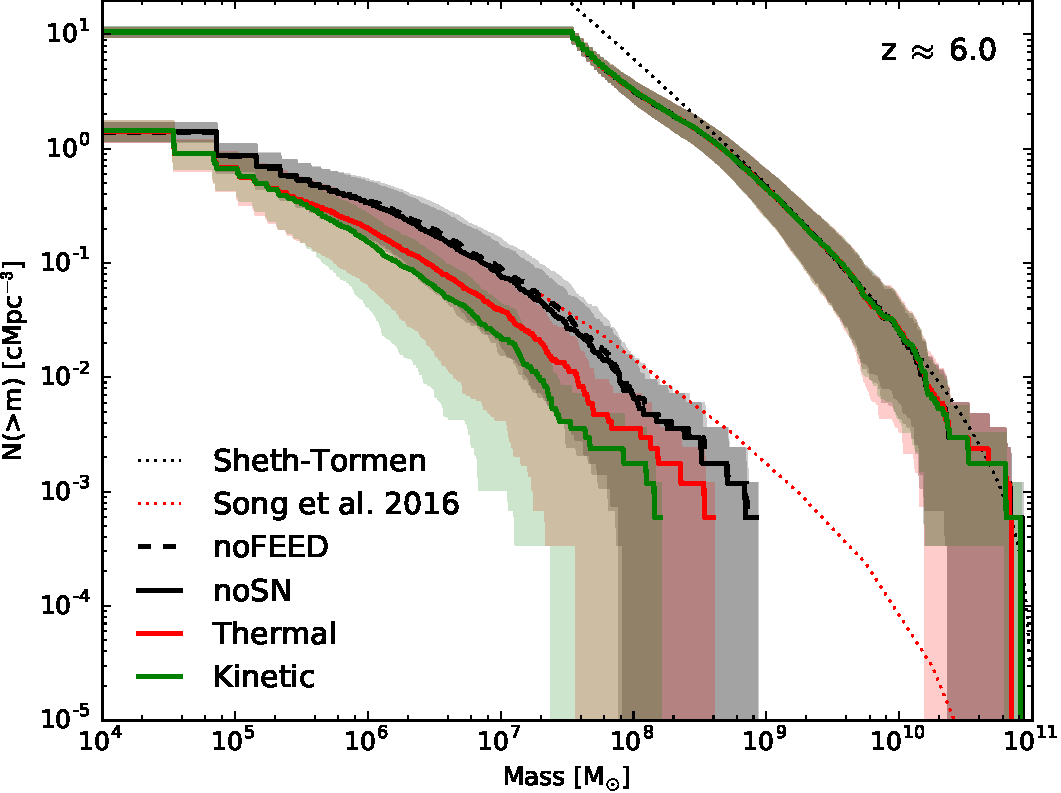
\includegraphics[width=.95\linewidth]{img/03/ghmf.pdf}
        \caption{Fonction de masse des galaxies (GMF) et des halos (HMF) pour différents type de feedback de supernovae.
        Le feedback n'a pas d'influence directe sur la function de masse des halos, mais a un impact mesurable sur la formation stellaire.
        }
 		\label{fig:ghmf}
\end{figure}



\subsection{La masse d'étoiles en fonction de la masse du halo}
Plus un halo est massif, plus celui ci va contenir d'étoiles.



\subsection{La formation stellaire en fonction de la masse du halo}
\label{sec:sfr_halo}
Connaissant, a un instant donné, les étoiles appartenant a chaque halo, il est possible de déterminer leurs ages, et donc de connaitre l'histoire de formation stellaire de chaque halo.
Nous allons voir que la masse 


\begin{figure}[bth]
		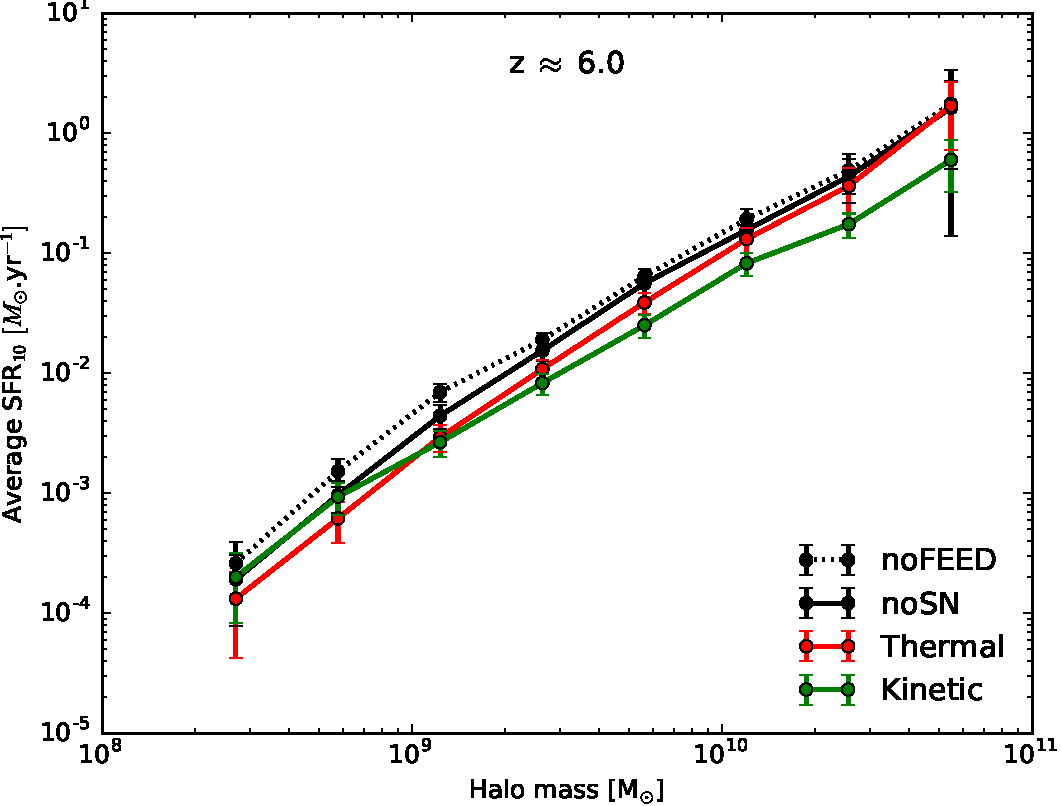
\includegraphics[width=.95\linewidth]{img/03/SFR_halo_avg.pdf}
		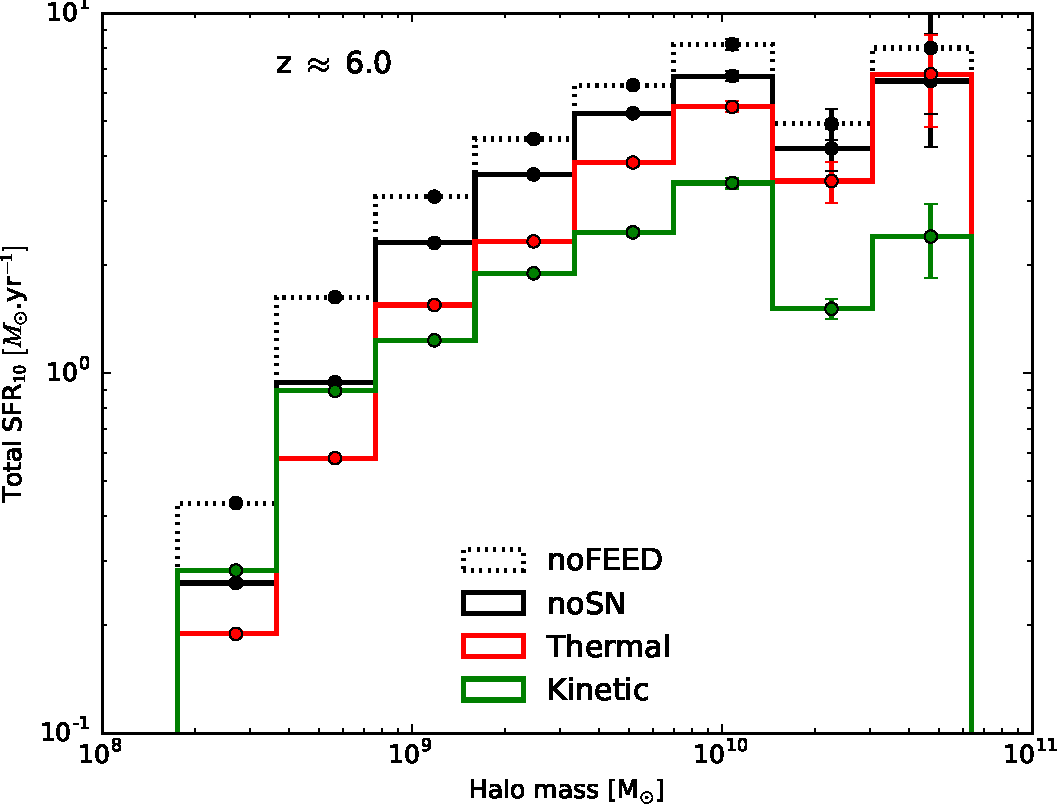
\includegraphics[width=.95\linewidth]{img/03/SFR_halo_tot.pdf}
        \caption{SFR en fonction de la masse du halo moyenne en haut et total en bas.
        }
 		\label{fig:sfr_halo}
\end{figure}



\subsection{La fraction baryonique}
\label{sec:baryon_frac}
La fraction baryonique est une grandeur importante pour caractériser un halo.
En effet, le rayonnement n'interagit qu'avec les baryons et plus un halo aura de baryon, plus le rayonnement aura de difficulté a s'en échapper.

\begin{equation}
f_b = \frac{M_* + M_{gas} }{M_{DM} + M_* + M_{gas} }
\end{equation}


\begin{figure}[bth]
		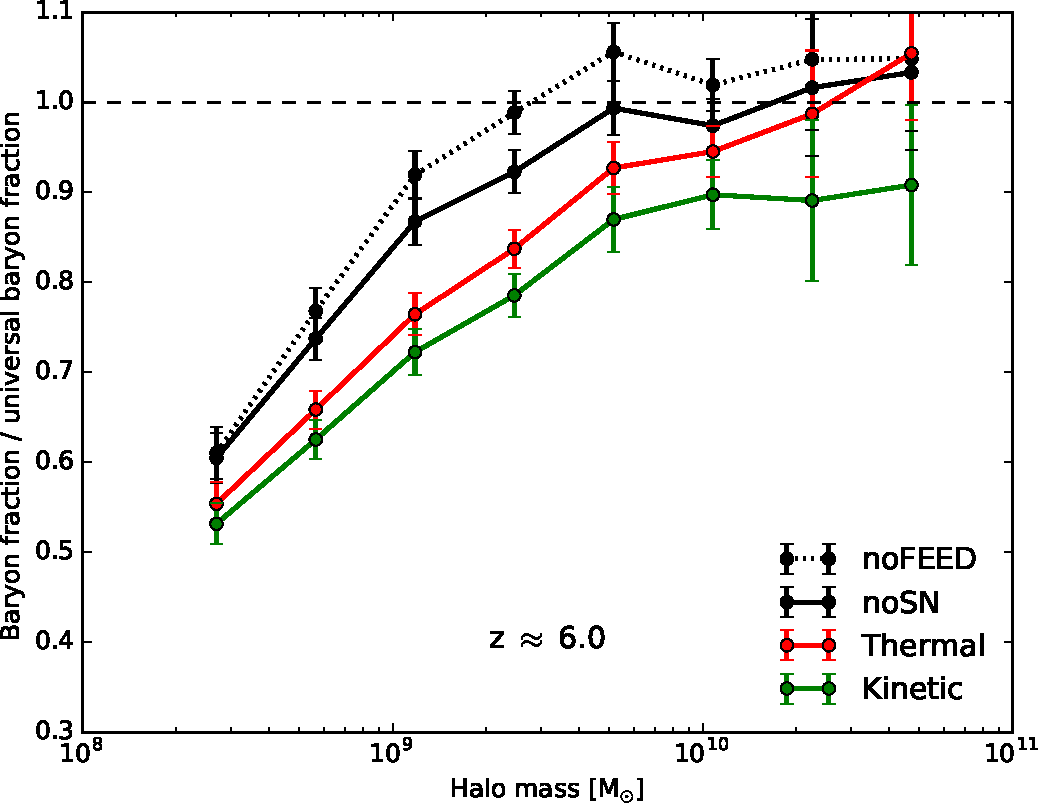
\includegraphics[width=.95\linewidth]{img/03/baryon_frac.pdf}
        \caption{Fraction baryonique en fonction de la masse du halo et des feedback.
        }
 		\label{fig:bfrac}
\end{figure}


La figure \ref{fig:bfrac} présente les résultats obtenus.



\section{Étude a la surface des halos}

Nous cherchons ici a quantifier les flux entrants et sortant des halos en fonction de leurs masses.
Nous présenterons la méthodologie utilisé pour la détection de ces flux, ainsi que les résultats obtenus pour les flux hydrodynamique et radiatif.




\subsection{Détermination des flux au $R_{200}$}
\label{sec:healpix}

Une question importante dans l’étude de réionisation est la quantité de rayonnement ionisant sortant des halos.
Nous avons vu que le rayonnement interagis les baryons, et nous verrons qu'il existe un liens entre la fraction baryonique déterminée plus haut (sec. \ref{sec:baryon_frac})
et les flux radiatif.


Nous cherchons a déterminer les flux a la surface des halos.
Par soucis de simplicité, nous utiliserons l'approximation du $R_{200}$.
Il faut donc discrétiser la sphère de rayon $R_{200}$.


\subsubsection{Healpix}
\label{sec:healpix}

Cette discrétisation de sphère sera réalisée grâce a Healpix \citep{gorski_healpix:_2005}.
Healpix est un outils qui permets de répartir des points de manière uniforme sur la sphere (c.f. figure \ref{fig:HealPix}).
L'avantage de cette méthode est que toutes les cellules ont la même pondération.


\begin{figure}[bth]
        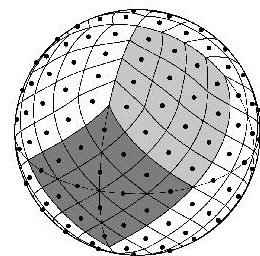
\includegraphics[width=.95\linewidth]{img/03/healpix.jpg} 
        \caption{Exemple de sphere HealPix}
 		\label{fig:HealPix}
\end{figure}

%L'association Healpix/grille sera réalisée par recherche de plus proche voisin 
Par la suite, les halos seront discrétisé en utilisant $3072$ point Healpix.
Une fois la sphère générée, on la centrera sur la position du halo, et on la redimensionnera de telle manière a ce qu'elle corresponde aux R200 du halo en question.
Puis, pour chaque point de la sphère Healpix, on effectuera une recherche de plus proche voisin à l'aide d'un KD tree, pour déterminer avec qu'elle cellule l'associer.


Nous avons donc accès aux cellules correspondant a la surface du halo.
%Nous connaissons maintenant l'ensemble des cellules au R200 de chaques halos.
Nous pouvons donc travailler directement avec les grandeurs scalaires.
Mais nous cherchons a réaliser une étude sur les flux.
IL sera donc nécessaire de projeter les vecteurs de flux sur la normale des cellules de la sphere.




%Pour déterminer les flux autours de chaque halo, il est nécessaire de les englober d'une sphère.
%Cette sphère serra discrétisée a l'aide de Healpix (TODO ref) un outils qui permets de répartir des points de manière uniforme sur une surface sphérique .



\subsection{La vitesse du gaz au $R_{200}$}

Dans le but de mettre en évidence l'efficacité des supernovae a expulser le gaz des halos, j'ai quantifié la vitesse moyenne du gaz autour des halos au niveau de leur R200.
Par convention, la normale a la sphère pointe vers l'extérieur.
Donc si la vitesse moyenne est positive, le halo perd de la matière baryonnique, et sinon il en accrète.
%TODO inserrer figure flux
Dans le cas idéal, la matière chute sur le halo à la vitesse de chute libre.

\begin{equation}
v_{lim} = \sqrt{\frac{2 GM (r<R_{200})} {R_{200}} } 
\end{equation}

A l'inverse, si de la matière est expulsé plus rapidement que cette vitesse limite, elle n'est plus gravitationnelement liée au halo.

En absence de feedback, la quasi totalité des halos se trouvent sur cette relation limite.
De part la nature collisionnelle des baryons, cette vitesse est une limite superieure, les baryons accrétés étant ralentit par la présence des baryons initialement prsent au sein du halo.

Un des résultat obtenu est qu'au moment de l'introduction de la radiation dans les simulation, il y a apparition d'une population de halo de faible masses avec des vitesses moyenne positives.
Dans ce cas, la radiation est en mesure de générer des flux sortant, et donc de diminuer la fraction baryonnique de cette classe de masse. $M<qq 10^8$.
Cette population ne possède pas d'étoile, ce qui suggère un effet extérieur au halo.
La vitesse d'expulsion moyenne est significativement plus faible que la vitesse d'échappement (1 ou 2 ordres de grandeurs).

De plus dans la partie accrétante du diagramme on observe que la vitesse limite est globalement plus faible (la population s'est légèrement écartée de la ligne limite).
Également, la dispersion des valeurs moyennes est plus grande, signifiant que la radiation n'agit pas de la même façon sur tout les halos.

Avec l'introduction des supernovae, il y a apparition d'une nouvelle population dans la partie haute du diagramme.
Cette population possède des étoiles aillant déjà exposées en supernovae, ce qui suggère un effet provenant de l'intérieur.
On observe que les halos possédant des vitesses positives peuvent avoir des masse plus élevées que dans le cas du simple feedback radiatif.
De plus, le feedback cinétique permet de générer des outflows sur des halos plus massif que dans le cas du feedback thermique.
Les vitesses moyennes sont proches de la vitesse d'échappement.

\subsection{Le flux radiatif au $R_{200}$}
%TODO inserrer figure flux

Comme dans ces simulations, la lumière est décrite comme une fluide (cf Sec. ) %TODO ref
Un travail identique a celui de la section précédente peux être réalisé sur les flux radiatif.

Nous observons que la quantité de photon s'échappant des halos ne dépend pas (ou tres peux) de la méthode de feedback de supernovae.

problème du coarserad %TODO ref
Résolution plus faible que pour l'hydro.
(résolution des CODA)




\subsection{Fraction d'échappement}

Par contre nous avons vu que le taux de formation stellaire et donc le taux de production de photon, dépend du modèle de supernovae (Sec. \ref{sec:sfr_halo}).
En comparant les flux radiatif sortant, a la production de photon interne au halo, il est possible de quantifier une grandeur centrale dans l'étude de la réionisation : la fraction d'échapement des photons.

Les emmisivité sont corrigées du temps necessaire au parcours des photons entre le centre du halo et son $R_{200}$.
%fonction de luminosité 


\section{Conclusion}


Nous avons vu dans cette partie différentes méthodes pour gérer les supernovae dans les simulations cosmologique.
Nous avons vu que la formation stellaire est fortement couplée a la méthode d'injection d'énergie.
Une injection d'énergie sous forme cinétique sera plus efficace pour réguler la formation stellaire qu'une methode thermique.
La régulation de la formation stellaire se fait par l'intermédiaire de l'expulsion des baryons des halos, privant ainsi les zone de formation de matière première.
Or, cette diminution de la quantité de baryon, permet a la radiation de s'échapper plus facilement.

Au final, la compétition entre la diminution du taux de production de photon et l'augmentation de la fraction d'échappement semble neutre.

Cette conclusion n'est valable qu'au résolution considérées dans cette étude, c'est a dire la résolution des plus grosses simulations de la réionisation comme CODA ou CROC. %TODO ref.

De plus nous observons que le budget de photons est principalement gouverné par les halos de masses intermédiaire. $10^{10} M_\odot$







